% !TEX TS-program = pdflatex
% !TEX encoding = UTF-8 Unicode

% This is a simple template for a LaTeX document using the "article" class.
% See "book", "report", "letter" for other types of document.
\documentclass[11pt]{article} % use larger type; default would be 10pt
\usepackage[utf8]{inputenc} % set input encoding (not needed with XeLaTeX)

% These packages are optional, depending whether you want the features they provide.

%%% PAGE DIMENSIONS
\usepackage{geometry} % to change the page dimensions
\geometry{letterpaper} % or letterpaper (US) or a5paper or....
\geometry{margin=1in} % for example, change the margins to 2 inches all round
% \geometry{landscape} % set up the page for landscape

\usepackage{graphicx} % support the \includegraphics command and options
\usepackage{hyperref}

\usepackage[parfill]{parskip} % Activate to begin paragraphs with an empty line rather than an indent

%%% PACKAGES
%\usepackage{booktabs} % for much better looking tables
\usepackage{array} % for better arrays (eg matrices) in maths
%\usepackage{paralist} % very flexible & customisable lists (eg. enumerate/itemize, etc.)
\usepackage{verbatim} % adds environment for commenting out blocks of text & for better verbatim
%\usepackage{subfig} % make it possible to include more than one captioned figure/table in a single float

%%% HEADERS & FOOTERS
\usepackage{fancyhdr} % This should be set AFTER setting up the page geometry
\pagestyle{fancy} % options: empty , plain , fancy
\renewcommand{\headrulewidth}{0pt} % customise the layout...
\lhead{}\chead{}\rhead{}
\lfoot{}\cfoot{\thepage}\rfoot{}

%begin the doc

\title{Introduction to Arduino}
\author{}
\date{} % Activate to display a given date or no date (if empty),

\begin{document}
\maketitle


\section*{Introduction}

Just adding a test edit...

%At this point, we have seen simple examples of how to measure something about our surroundings using an oscilloscope  (e.g., temperature) and how to change something (e.g., using a heater to warm up our enclosures).  But all of these experiments were done `manually' -- you turned on a voltage supply or read the temperature from a data stream. What we're missing is \emph{control}.

With the proliferation of modern microcontrollers, control of electromechanical systems has moved from dedicated circuitry and specialized hardware to more general implementations where a small computer -- the microcontroller -- is programmed to work with various sensors and actuators using high-level languages (e.g., C or python). One of the primary benefits is that microcontrollers are very flexible, and that flexibility allows the designer to quickly change parameters and try them out without having to significantly redesign the system hardware.

Here, you will be introduced to the Arduino, a low-cost prototyping platform based on the ATmega328P microprocessor from Atmel, fine purveyors of microcontrollers since 1984\footnote{and recently bought out by Microchip, fine purveyors of microcontrollers and electronics since 1987.}. The makers of Arduino have taken several Atmel processors and built a platform around them that simplifies programming, communication, power management, and interfacing with peripherals. You will eventually use the Arduino to do many tasks; in this lab and the next, you’ll learn about the architecture of the Arduino, write some basic programs, and build a handful of fundamental circuits.

\section*{Inventory}
\label{sec:inventory}

All of your materials will be checked out from the Rice 120 Microcontroller Library using the high-tech, bar-code checkout system (props to Danny Voce, TLP third-year, for his work setting this up!). An explanation of the system will be provided during the first lab meeting. Your team will be given a plastic bin to maintain all of your supplies. An official inventory of what you should (and should not!) have in your bin is linked on collab. Keep in mind that this inventory will grow throughout the term as you implement more and more components. Also keep in mind that there are a number of contraband items that you may not keep in your bin -- communal items such as DMMs and such. Your team will receive demerits if I find contraband in your bin -- accrue enough demerits and it will affect your grade.

The core of your supplies is a SparkFun Inventor’s Kit. A complete description of the kit and its components can be found at the \href{https://www.sparkfun.com/products/12060}{\underline{SparkFun Inventor’s Kit}} webpage. There is also a reference sheet in the kit, which also has a list of components. There is also a large experimental board with a large breadboard and some switches and knobs. You will also have a red, plastic box to hold minor electronics. You will be given jumper wires and breadboard wires (they have different uses!). Poor wiring techniques will not only make your system more prone to errors, but will lead to sarcasm and derision from your instructor. If your wiring is particularly bad, your instructors will refuse to help you troubleshoot.

\section*{The Arduino Uno}

Throughout the term, your team will make frequent use of a SparkFun RedBoard, an authorized\footnote{Anyone can clone an Arduino -- they’re open source -- but only those who work with Arduino directly can use the Arduino trademark} clone of the Arduino Uno, as well as a wide-variety of electronics: sensors, actuators, and other peripherals. In this class, we will use the terms “Arduino Uno” and “SparkFun RedBoard” interchangeably -- the only practical difference is the USB port. In later labs, you will have a chance to “branch out” from the basic Arduino Uno to some more powerful microprocessors (e.g., Atmel’s SAMD21 ARM chip). 

\subsection*{The Arduino IDE}

%\subsubsection*{Programming}

The Arduino programming language is essentially C++ (a predecessor to java), with a few caveats. First and foremost is that instead of a \verb|main()| as an entry point, all Arduino programs, often called \emph{sketches}, have a \verb|setup()| function and a \verb|loop()| function. When the program starts, \verb|setup()| is run once, and then the program loops through \verb|loop()| indefinitely. That is, you never really ``end'' a program in Arduino, though you can add an infinite, do-nothing, \verb|while()| loop if you want it to stop doing anything useful. 

The Arduino environment provides a number of libraries, some “built-in”, some “added-on”, to perform a number of common functions. For example, the 328 has several analog-to-digital channels that can be used to read voltages from a sensor (more on this below). Performing the conversion using chip instructions is a bit complicated, so the Arduino environment wraps all the details into a single function, \verb|analogRead()|. The main advantage to this framework is obvious, but the simplicity comes at the cost of efficiency -- because they are generic, library functions are generally slower than calling the chip commands themselves. Much of the time, the cost in efficiency is hardly noticed, but occasionally you need to dig deeper into the hardware to extract all the power you can.

Another drawback is that the libraries can be memory hogs. The ATmega328 microprocessor has only a little over 32kB of program memory to work with and only 2kB of RAM(!), and all it takes is two or three poorly written libraries to consume one or the other. On top of that, memory issues can be very hard to diagnose, and the addition of debug statements will only exacerbate the problem. Still, you shouldn't have any problem with the basic projects we'll do in this class. For more advanced systems, we’ll use a more powerful processor with more RAM. \footnote{Your professor learned how to program on a TRS-80 -- look it up -- which had a whopping 4kB of memory. Kilobytes. Not Giga. Not Mega. Kilo. Kids have it so easy these days.}

\subsubsection*{The bootloader}

Most modern microcontrollers manage programming with something called a \emph{bootloader}, a small program that allows the user to run loaded programs or upload new ones. The bootloader lives on the microprocessor and is automatically run anytime the chip is powered up or reset. The bootloader will then listen to the programming port to see if the user is attempting to load a new program. If so, the bootloader loads the program, stores it, and runs it. If not, it runs whatever program was previously loaded. That is, programs are stored in persistent flash memory, so when you first power up an Arduino, \emph{it runs the most recently uploaded program.} This can be particularly bad if your last sketch did something unwise, such as connect an output pin directly to ground.

\subsubsection*{Serial Monitor}

One drawback of the Arduino IDE is that it has no debugger. Your primary means of debugging, as well as getting information to and from your computer, is through the Serial Monitor. To start the serial communication on the Arduino, you need to add \verb|Serial.begin([speed])| to the \verb|setup()| function, where \verb|[speed]| is the \emph{baud rate} of the communication. Often, a baud rate of 9600 bits/second (bps) is used. If you need to send faster data, you can easily go as high as 115200 bps. To write data to the Serial Monitor, use \verb|Serial.print()| or \verb|Serial.println()|, the latter of which adds a newline character to the end. Note that the Serial class is not very `smart' -- you can't concatenate things easily, so you will often end up putting lots of \verb|Serial.print()| lines in. {\bf If you want your instructor to help you debug something using the Serial Monitor, you must format the output nicely!} This generally means putting related output on a single line, separated by tabs (\verb|’\t’|) or commas. Poorly formatted output will be met with sarcasm and derision.

On the computer side, you can open a Serial Monitor by pressing F12 or clicking on the icon near the upper right of the IDE. Note that doing so will send a reset command to the Arduino, so your program will start over. You'll need to set the communication speed to the same that the Arduino is using. If you get gibberish, you almost certainly have two different baud rates. It's possible to send data from the computer to the Arduino, as well, but we won't use that function in this handout.

With the Arduino Uno, communication to the computer does not happen directly. Your computer is connected to the Uno using a USB connection, but the ATmega328 cannot process USB communication directly. Instead, a second chip -- FTDI’s FT231XS on the RedBoard -- is used to translate from “USB-speak” to a protocol the 328 can understand. This protocol uses something called a \verb|UART|. We’ll get into the details later, but the important thing to note is that the \verb|UART| on the 328 is connected to pins 0 and 1 on the Uno. {\bf If you use the Serial Monitor, you will almost certainly not want to use these pins for anything else!}

\section*{Tutorials}
\label{sec:tutorials}

The following tutorials will cover two standard microcontroller functions: digital output and digital input, as well as getting you started on programming. We’ll discuss more about the differences between “digital” and “analog” in class. You may complete these tutorials during the first lab period, time permitting, or on your own time. In either case, {\bf you must complete them as a team.} You should have plenty of opportunities in the first week of classes to meet as a team.

If you’d like more tutorials, the SparkFun website has many to help you get started. You’re welcome to ask your instructor for suggestions. One tutorial that many beginners find useful is how the breadboard is used. You can find that \href{https://learn.sparkfun.com/tutorials/how-to-use-a-breadboard}{\underline{here}}.

\subsection*{A note on Input/Output}

In these tutorials, you will only be using digital I/O. Note, however, that all of the pins on the Arduino can be used for digital I/O, including the “analog” pins A0 - A5. A digital pin can be set as either an \verb|INPUT|, which allows the user to read an external device or as an \verb|OUTPUT|, which allow the user to control an external device. The command \verb|pinMode()| is used to set the mode of the pin to one of three options:\footnote{These modes apply to most microcontrollers, not just the ATmega, though the specific methods will vary.}

\begin{itemize}
\item {\bf OUTPUT}. When configured as an output pin, the pin will either source or sink current \emph{with essentially zero resistance.} It is therefore {\bf very important} to calculate the current that will flow to or from the circuit to which the pin is attached. If the equivalent resistance of the circuit is low, large amounts of current can flow through the pin, damaging the Arduino. \emph{It is extremely important that you never connect an output pin directly to GND or 5V or any other pin that could cause a short circuit.} The command \verb|digitalWrite()| is used to set the pin to a \verb|HIGH| or \verb|LOW| voltage.
\item {\bf INPUT}. When set as an \verb|INPUT|, the user can read the pin using \verb|digitalRead()|, which return ‘0’ if the voltage on the pin is low and ‘1’ if the voltage is high. The exact thresholds are left for the student to determine. If nothing is attached to the pin, very small currents, such as the static discharge of your finger, can effectively change the voltage of the pin. When this is the case, the pin is said to “float” -- repeatedly reading the pin will produce essentially random HIGHs and LOWs. Another important thing to note is that the impedance (a fancy word for “resistance”) of the pin will be extremely high -- on the order of $100M\Omega$. This means that essentially no current will flow into or out of the pin when it is declared an input.
\item {\bf INPUT\_PULLUP}. In this configuration, the pin is set as an input pin (as above), but it is \emph{internally} connected to a $20k\Omega$ pull-up resistor. This allows you to prevent floating inputs without having to wire up additional circuitry. More on that later.
\end{itemize}

Note that it is possible to switch between modes while a program is running by simply making repeated calls to \verb|pinMode()|. Also, by default, all pins start as inputs, so there is no need to explicitly set a pin to be an input, though it is good practice to do so.

\subsection*{Timers}

There are several ways to measure time in Arduino. The ATmega chip has three 8- and 16-bit \emph{hardware timers} that can be used for low-level timing functions, such as pulse width modulation or synchronizing communications. At the lowest level, the \emph{system clock} runs at 16MHz and controls all of the hardware timers, which can be configured for a variety of tasks. Luckily for us, the makers of Arduino have harnessed the power of these hardware timers into easy-to-use software functions. For timing purposes, the most useful functions are,
\begin{itemize}
\item \verb|millis()|, which returns an \emph{unsigned}, 32-bit integer that represents the number of milliseconds since the program started. After the value reaches its maximum (what value is that?), the return value “rolls over” to 0 after the next millisecond. Note that subtraction of two calls to \verb|millis()| works even when the clock has rolled over.
\item \verb|micros()| works just like \verb|millis()|, but returns the number of microseconds.
\item \verb|delay()| can be used to pause the program for a given number of \emph{milliseconds}. Note that the Arduino won’t be able to do anything else while it’s in the \verb|delay()| function\footnote{Interrupts excepted -- more on that another day.} -- it is a \emph{blocking} function -- so \verb|delay()| is really only useful for short pauses when nothing critical could happen. In general, \verb|delay()| is frowned upon except for the most basic programs. You will eventually use event-driven programming to time events without blocking execution of the program.
\item \verb|delayMicroseconds()| is just like \verb|delay()| but takes an argument in microseconds. Note that it only works in steps of 4 $\mu s$.
\end{itemize}

More information about these functions can be found on the Arduino website. In a future lab, you will use them to write an \emph{event-driven} timer.

\section*{Digital output}
\label{sec:digital.out}

\subsection*{Procedure}
\begin{enumerate}
\item Complete \href{https://learn.sparkfun.com/tutorials/sik-experiment-guide-for-arduino---v32/experiment-1-blinking-an-led}{\underline{Experiment 1: Blinking an LED}}, the Arduino equivalent of “Hello, World!”.

There are a couple of important things to note:
\begin{itemize}
\item Digital pins (0-13) can be declared as either \verb|INPUT| or \verb|OUTPUT| or \verb|INPUT_PULLUP| (default is \verb|INPUT|), and you can change the pin mode while the program is running. When set to \verb|OUTPUT|, a \emph{digital} pin can be set to either \verb|HIGH| (5 V) or \verb|LOW| (0 V). Note that the pins can only tolerate 40mA -- \emph{milli}amps -- of current before you risk damaging them, and in most cases you’ll want to limit the current to far less. Therefore, \emph{it is essential that you determine how much current is expected to flow through an output pin before you power your Arduino.} {\bf Under no circumstances should you connect an output pin directly to 5V or GND}, as you will almost undoubtedly burn the pin out. It's usually a good idea to include a resistor (at least $220\Omega$) on output pins where it won't affect the operation of the rest of the circuit, just in case the rest of circuit has a short in it. 
\item On that note, what do you think the resistor in the LED circuit is for? Say you measured the voltage drop across the LED and found it to be 1.4V. How would you calculate how much current is running through it?

\end{itemize}
\item Adjust the delays in the code such that the LED is on for 2 seconds and off for 0.5 seconds and reload the code.
\item Without changing your code, rewire the circuit as shown in Figure~\ref{fig:led.reverse}. {\bf Be sure to remove the GND wire to avoid a short circuit!} How long is the LED on now when you run the program? Why? Is pin 13 sourcing or sinking current?

\begin{figure}[htbp]
\begin{center}
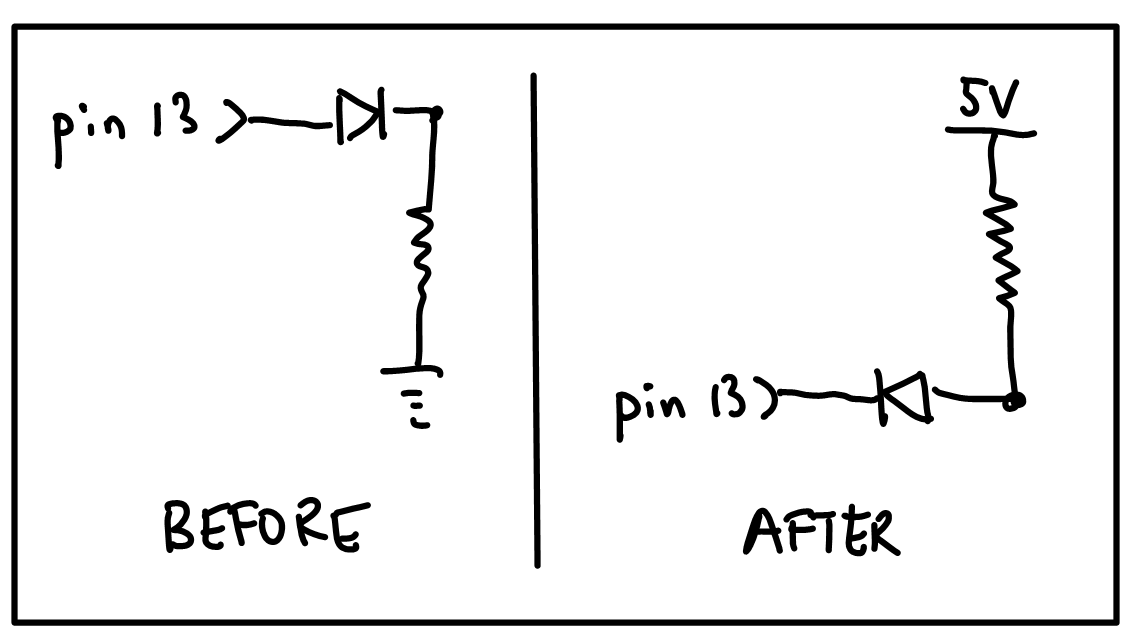
\includegraphics{figures/led_reversed}
\caption{A different LED circuit.}
\label{fig:led.reverse}
\end{center}
\end{figure}

\end{enumerate}

\section*{Digital input}
\label{sec:digital.in}
\subsection*{Procedure}

\begin{enumerate}
\item Complete \href{https://learn.sparkfun.com/tutorials/sik-experiment-guide-for-arduino---v32/experiment-5-push-buttons}{\underline{Experiment 5: Push Buttons}}.

The most important thing to note is the use of \emph{pull-up resistors}. When a pin is set to input mode, it is connected internally to a very large resistance ($>100M\Omega$). Because of this, it doesn't take much current to flip the pin from reading \verb|HIGH| to \verb|LOW|; without the pullup resistor, when the button is open (up), noise, stray currents, your finger all would make the state jump back and forth between \verb|HIGH| and \verb|LOW| seemingly randomly. To combat this undesirable behavior, you can employ a pull-up resistor. This loosely connects the input pin to 5V so that when the button is open (up), the input pin will always read \verb|HIGH|. When the button is closed (down), the pin is connected directly to ground, which brings it \verb|LOW| (as an input pin, it is OK to connect the pin directly to GND). We call this an example of \emph{inverted logic}.

\item Note that a small amount of current flows from 5V to ground through the pull-up resistor when the button is pressed. How much?
\item Remove the pull-up resistor. Rub your finger on the breadboard near the button. Does the LED flicker, indicating random changes in the button state? Edit your code and declare the pin mode to be \verb|INPUT_PULLUP|. All should be well again!
\item Finally, edit your code so that pressing the button on pin 2 turns the LED on, and pressing the other button turns it off. For this you will want to use a format like: 

\verb|if button A is pressed => turn the LED on|\\
\verb|if button B is pressed => turn the LED off|

\end{enumerate}

\clearpage
\section*{Tutorial Worksheet (5 points)}
\label{sec:prelab}

{\bf To be turned in Wednesday, Jan. 24 at the start of class.} One per team.

\emph{Answers with incomplete or incorrect units will be marked as wrong!}

\begin{enumerate}

\item Give 10 examples of every day devices that incorporate microprocessors, microcontrollers, or DSPs.
\vspace{1.75in}
%\item Given the voltage divider circuit in Figure~\ref{fig:voltagedivider}, determine the voltage at point B if $R_1 = 680\Omega$ and $R_2 = 2.2k\Omega$. Use $V_A = 5V$ and $V_C = 0V$.
\vspace{1in}
\item What is a \emph{floating input}? How do we combat them?
\vspace{1in}
\item With an Arduino powered at 5V, what is the voltage threshold above which a digital input is \emph{guaranteed} to produce a HIGH reading?
\vspace{0.5in}
\item What is the largest number that can be returned by \verb|millis()|? {\bf Be exact.} Roughly how long will it take to roll over (from 0 all the way back to 0)?
\vspace{0.25in}
%\item In the oscilloscope image in Figure~\ref{fig:trigger}, what trigger settings are being used (source, condition, and level)?
%\vspace{0.75in}
%
%\begin{figure}[htbp]
%\begin{center}
%%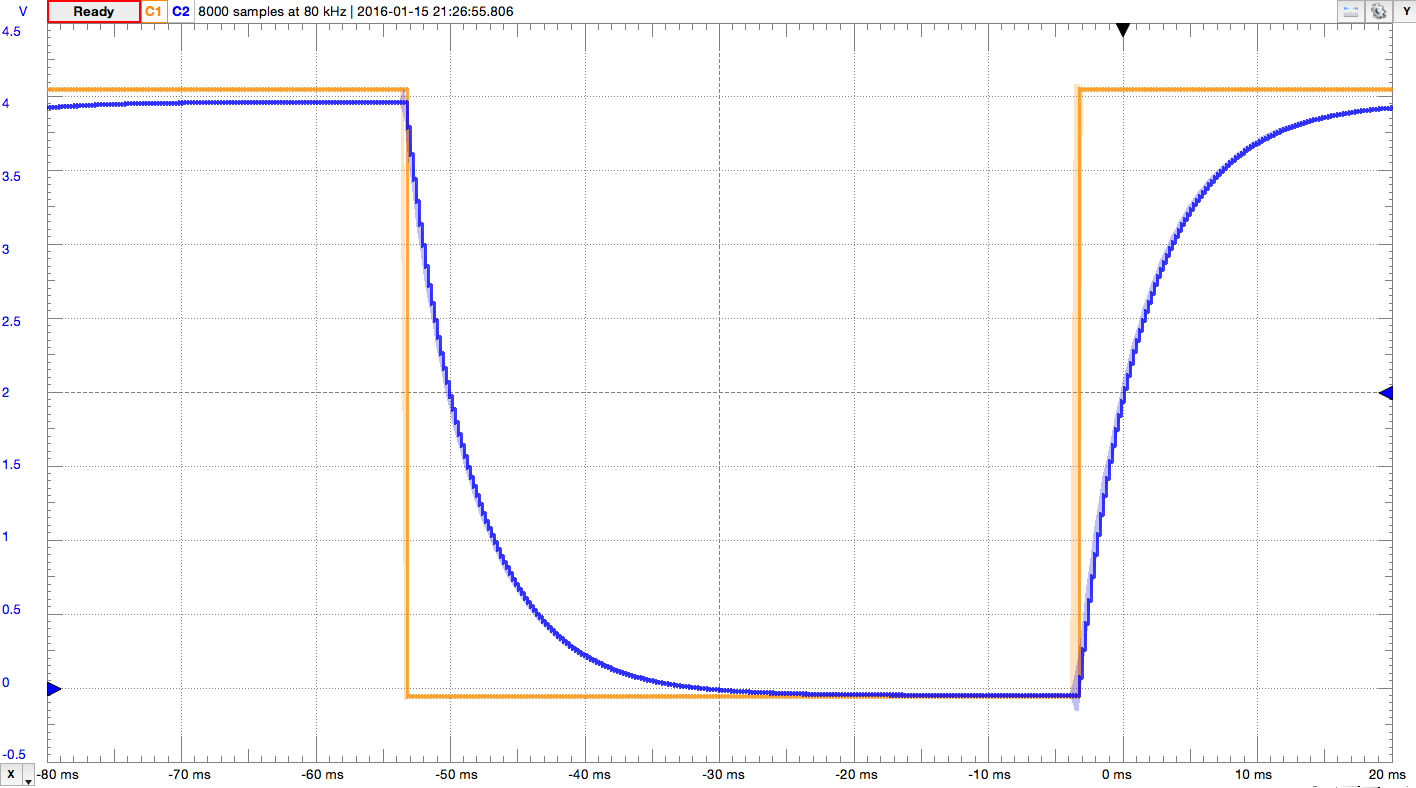
\includegraphics[width=\textwidth]{figures/rc_capture}
%\caption{A oscilloscope capture from an RC circuit.}
%\label{fig:trigger}
%\end{center}
%\end{figure}
%
\item Current through the LED in Experiment 1: \rule{2in}{0.4pt}
\vspace{0.25in}
\item Current through the $10k\Omega$ pull-up resistor: \rule{2in}{0.4pt}
\vspace{0.25in}
\item Why do you use a fairly large resistor for a pull-up? 
\vspace{0.25in}


\item Attach your code for turning on and off the LED with the two buttons.
\end{enumerate}

\end{document}
